\documentclass{article}
\usepackage{latexsym}
\usepackage{amssymb,amsmath}
\usepackage{custom2}
\usepackage{graphicx} % for figures
\usepackage{epstopdf} % so can use EPS or PDF figures
\usepackage{caption}
\usepackage{subcaption}
\usepackage{url}
\usepackage{amssymb,amsfonts}
\usepackage[all,arc]{xy}
\usepackage{enumerate}
\usepackage{mathrsfs}
\usepackage{booktabs}
\usepackage[pdftex]{hyperref}
\usepackage{lscape}
\usepackage{xcolor}
\usepackage{natbib}

\captionsetup{justification=RaggedRight, singlelinecheck=false}
\newcommand{\ra}[1]{\renewcommand{\arraystretch}{#1}}
\newcommand{\argmax}{\text{argmax}}
\newcommand{\Tr}{\text{Tr}}
%\newtheorem{claim}{Claim}
\newtheorem{ass}{Assumption}

\addtolength{\evensidemargin}{-.5in}
\addtolength{\oddsidemargin}{-.5in}
\addtolength{\textwidth}{1.4in}
\addtolength{\textheight}{1.4in}
\addtolength{\topmargin}{-.5in}

\pagestyle{empty}

\begin{document}
\begin{center}
\Large

\end{center}


\vspace{0pt}

\begin{center}
{\bf \LARGE{Stochastic Learning Dynamics with Two Applications}}
\end{center}

%\tableofcontents

\section{Abstract}
%Learning usually occurs in noisy environments.  In order to make a decision, one must accumulate the  evidence for different alternatives and choose one only once the uncertainty about the choice is sufficiently reduced.  There are two biological systems in which the variables used to make a decision can be described by a random walk: the firing rates of neural populations in the brain of an individual making a decision about a visual stimulus and the beliefs of monkeys about their relative dominance based on the fights they have engaged in.  The same stochastic differential equations can be used to model these quite different systems, which suggests that there are universal principles underlying learning through noisy dynamical systems.  In the neural system, the differential equations are often reduced to a one-dimensional model, but the social system is inherently two-dimensional.  The thresholds dictating when a decision has been made affect both the accuracy of the decision and the expected time until a decision is reached. We find that the dimensionality of the decision process does not affect its accuracy.  We find that if a pair of individuals optimize their thresholds to avoid waiting, a pair making an easy decision will take more time than a pair making a difficult decision.  In a group of individuals optimizing their thresholds to avoid waiting, those pairs making the difficult decisions about high value inputs will have to wait the longest.  Finally, the skewness of the power distribution in the social system is maximized at intermediate waiting costs and the information content of the power distribution is higher when the individual maximize their probability of becoming dominant rather than the accuracy of their decisions. In comparing the output of the model of the social system to data, we found that ...

\section{Introduction}

Collective computation

decision making previously and why social systems are different

specifically, how do monkey groups compute their power structure?

the model, which extends neural models, reduces to game theory, and can be derived from first principles with only a few assumptions!  aren't we great?

\subsection{Neural }
Stochastic differential equations have been used to model, explain, and predict learning and decision making in both monkeys and humans \citep{Eckhoff:2008uq, Brown:2005fk,Feng:2009kl,Bogacz:2006uq}.  Typically, an experimental subject is presented with a visual stimulus that consists of dots, some percentage of which are moving coherently either left or right and the rest of which are moving randomly.  The subject is then asked to decide in which direction the dots were moving.  If there are two neural populations, each of which fire in response to a particular direction of motion, the firing rates of the two populations will tend to increase or decrease, depending on the strength and direction of the stimulus.  Eventually, either the experimenter forces a decision to be made, in which case whichever population has a higher firing rate determines which decision is made, or the firing rate of one population becomes high enough that the subject decides for that direction.  To summarize, there are two decision variables--- the firing rates of two neural populations responding to left and right motion--- that perform a biased random walk until enough evidence has been accumulated to make a decision one way or the other.


\subsection{Social }
In groups of pigtailed macaques, different animals have different fighting abilities, and when a pair of animals engages in a fight, one animal may be more likely on average to ``win" the fight.  Over time, as one animal learns that it is likely to lose fights, it will decide to emit a formal subordination signal, communicating its agreeing to the subordinate role in their relationship \citep{Flack:2007kx, Flack:2006fk,Flack:2004oq, Waal:1985fk,Caldecott:1986uk}.  The outcome of a fight is affected by each animal's allies, the presence of those allies, motivation levels,  external environmental variables, and other factors.  Additionally, the number of fights that occur in any period of time depends on similarly stochastic factors.  Because of this stochasticity, the number of fights won and lost in any period of time is a random variable.  Each animal's opinion about its relative dominance, therefore, will perform a biased random walk until one animal's opinion of itself is low enough to agree to being subordinate.  A similar model has previously been applied to animal conflicts, although in that case the model assumed that the animals had perfect memory of their past interactions \citep{Froment:2010fk}.


\section{The model \label{derivation}}
\subsection{Stochastic differential equations }
Learning systems have been successfully modeled with stochastic differential equations \citep{Eckhoff:2008uq, Brown:2005fk,Feng:2009kl,Bogacz:2006uq}, although the application of this type of model has been quite phenomenological.  With two assumptions about the timescales on which probabilistic events occur, a simple mechanistic description of the accumulation of information about random events can be turned into a stochastic differential equation \cite{Gillespie:2000fk}.  

%note about applicability to quorum sensing

In the absence of any input, the decision variables leak back towards $0$ with rate $\ell$.  (A table of all variables used in the text is given in Table \ref{variables}.)  If there is no input, then over a period of time of length $\tau$ a decision variable would decrease as $X(t+\tau)=(1-\ell\tau)X(t)$.  There are two types of inputs: in the neural system, a dot can move either left or right and in the social system a fight can be won by one animal or another.  For clarity in the following we will refer to these left or right dots, but the biological interpretation of the two types of inputs depends on the system.  Each decision variable responds positively to one type of input and negatively to the other, with the signs of their responds the opposite of each other.  Specifically, in the neural case, one neural population responds positively to left dots and negatively to right dots and the other neural population does the opposite.  In the social case, one animal's estimate of its own dominance increases when it wins fights and decreases when it loses fights, and the other animal's estimate does the opposite.  

To determine the estimate at time $t+\tau$, we can count how many times each of type of input occurred in the time since $t$ and add the changes resulting from these events to the background leaky estimate (as in \cite{Gillespie:2000fk}):
\begin{align*}
X_1(t+\tau)&=(1-\ell\tau)X_1(t)+b\times\# \text{ of left dots in }[t,t+\tau)-b\times\# \text{ of right dots in }[t,t+\tau)
\\ X_2(t+\tau)&=(1-\ell\tau)X_2(t)-b\times\# \text{ of left dots in }[t,t+\tau)+b\times\# \text{ of right dots in }[t,t+\tau). 
\end{align*}
where $b$ is the change caused by a single input.

Our first assumption is that the rates at which the two types of inputs occur is constant.  We can thus describe the number of each type of event with a Poisson random variable, $N_\text{L}$ and $N_\text{R}$.  We rewrite our basic equations to give 
\begin{align*}
X_1(t+\tau)&=(1-\ell\tau)X_1(t)+bN_\text{L}-bN_\text{R}
\\ X_1(t+\tau)&=(1-\ell\tau)X_2(t)-bN_\text{L}+bN_\text{R}.
\end{align*}
If events happen at a rate $r$ and the event is a left dot with probability $c$ and a right dot with probability $1-c$, then the expectation of $N_L$ and $N_R$ in a period of length $\tau$ are, respectively, $\tau r c$ and $\tau r(1-c)$. In the neural case, $c$ is related to the ``coherence'' of the visual stimulus.  A $c$ close to $0$ or $1$ means that most of the events are of one type or the other and the decision is easier to make than when $c$ is close to $.5$.

If enough events happen in the period of time from $t$ to $t+\tau$ then we can approximate the Poisson random variables with Normal random variables with mean and variance equal to the mean of the Poisson random variables.  Our second assumption, then, is that the period of time of length $\tau$ is long enough to make this approximation. Let $Z_\text{L}$ and $Z_\text{R}$, be independent standard Normal random variables, i.e. with mean $0$ and standard deviation $1$.  Then our equations for $X_i(t+\tau)$ become
\begin{align*}
X_1(t+\tau)&=(1-\ell\tau)X_1(t)+b\bigg(\tau rc+\sqrt{\tau rc}Z_{\text{L}}\bigg)-b\bigg(\tau r(1-c)+\sqrt{\tau r(1-c)}Z_{\text{R}}\bigg)
\\X_2(t+\tau)&=(1-\ell\tau)X_2(t)-b\bigg(\tau rc+\sqrt{\tau rc}Z_{\text{L}}\bigg)+b\bigg(\tau r(1-c)+\sqrt{\tau r(1-c)}Z_{\text{R}}\bigg).
\end{align*}
Finally, as we make the period of time shorter and shorter, making $\tau$ infinitesimally small, these equations become stochastic differential equations,
\begin{equation}
\begin{array}{ll}
dX_1&=\bigg(-\ell X_1(t)+br(2c-1)\bigg)dt+\bigg(b\sqrt{rc}\bigg)dW_\text{L}t-\bigg(b\sqrt{r(1-c)}\bigg)dW_\text{R}t
\\dX_2&=\bigg(-\ell X_2(t)-br(2c-1)\bigg)dt-\bigg(b\sqrt{rc}\bigg)dW_\text{L}t+\bigg(b\sqrt{r(1-c)}\bigg)dW_\text{R}t
\end{array}
\end{equation}
where $dW_{\text{L}}$ and $dW_{\text{R}}$ are independent Brownian motions representing, respectively, the left and right inputs.  The assumptions about the timescales on which inputs occur are particularly reasonable in the social system, although the successful application of this type of model to neural populations implies they are not unreasonable in that system.  In Table \ref{variables}, we list the inputs, outputs, and variables of the decision model and how they should be interpreted in the neural and social systems.


\subsection{Reaching a decision }
Each decision variable, $X_1$ and $X_2$, accumulates information about the stimulus.  The sign and size of the two variables indicate how much evidence there is for each possible decision outcome.  When a lot of evidence for the first possibility has been observed, $X_1$ will be large and positive, and similarly for the second possibility.  If the difference in the variables can be observed, the difference indicates the relative strengths of the evidence for either possibility. If $Y=X_1-X_2$, when $Y$ is large enough the system decides on $X_1$ and when $Y$ is low enough the system decides on $X_2$.  Specifically, there are two thresholds, $T_2$ and $T_1$ such that if $Y>T_1$ the decision is for $X_1$ and if $Y<-T_2$ the decision is for $X_2$.  However, it may be the case that the difference in the variables cannot be observed.  In this case, the decision depends on whether $X_1$ or $X_2$ hits a threshold first.  Again, there are two thresholds, $T_2$ and $T_1$, and if $X_1<-T_1$ the decision is for $X_1$ and if the $X_2<-T_2$ the decision is for $X_2$. 

In the neural system, the two stochastic equations describing the activity of the two neural populations integrating environmental evidence are often reduced to the one-dimensional equation describing the difference in the activity levels to make the system easier to analyze \cite{Brown:2005fk,Bogacz:2006uq,Feng:2009kl}.  However, in the social system we are considering, we cannot make any assumptions about the existence of a third party evaluating the difference in the opinions of the two animals.  A ``decision," i.e. the emission of a signal from one of the two animals, is only reached when one of the two animals' opinions goes below a certain threshold.  The social system is therefore inherently two-dimensional, whereas the neural system may be adequately described by one dimension.  In Table \ref{differences}, we compare how the decision is made and how the decision process is optimized in the two systems.

\subsection{Utility of the decision }
The thresholds affect the expected time until a decision is reached (decision time, DT) and the probability that an incorrect decision is made (error rate, ER).  The thresholds also affect the probability that either variable will ``give up'' first.  In the social case, this is the probability that each animal will emit a subordination signal (signaling probability, $\text{SP}_i$).  In the neural case, ??? These quantities, DT, ER, and $\text{SP}_i$, satisfy partial differential equations with respect to the starting values of the decision variables. In Appendix \ref{pdes_deriv}, we derive these partial differential equations.  While an analytical solution is known in the one-dimensional case, the two-dimensional case is analytically intractable.  We therefore numerically solve the PDEs in the two-dimensional case.  

The quality of the decision process depends on each of these three quantities.  The lower the decision time and error rate, the better the decision.  However, both cannot be decreased simultaneously so there is a tradeoff that depends on how the two quantities are prioritized.  Additionally, in the social case, each animal may benefit from lower its signaling probability, which may or may not conflict with lowering the error rate, depending on whether the animal is weaker or stronger than its opponent.  To quantify the utility of the decision process, we introduce three weights, $w_1$, $w_2$, and $w_3$, which determine how the three quantities are prioritized.  For animal $i$, we define
\begin{equation*}
U_{i}=w_1\text{DT}+w_2\text{ER}+w_3\text{SP}_i.
\end{equation*}
The decision is better if $U_i$ is lower.  In the social system, $w_2$ can be interpreted as the cost of fighting since when $w_2$ is higher, the time spent fighting until a decision is reached is more costly.  Similarly, $w_3$ can be interpreted as the benefit from being the dominant animal in a pair.


%A drift diffusion model is equivalent to a sequential probability ratio test, a learning algorithm that is optimal with respect to its accuracy and the time required to make a decision \cite{Moehlis:2004fk,Bogacz:2006uq}.  

\subsection{Optimal thresholds }
An individual-- either a neural population or a monkey-- can be engaged in either a single decision or in many decisions at once.  In the social system, for example, an animal wants to decide whether it is dominant or subordinate to every other member of its social group.  For any pair of individuals, each has a utility, $U_1$ and $U_2$, and consequently each has a Nash equilibrium threshold such that, if they choose those thresholds, neither has an incentive to choose another.  Similarly, in a group of individuals, each animal $i$ has a utility $U_{ij}$ from its decision process with animal $j$.  These lead to an optimized set of thresholds such that no individual has an incentive to choose another threshold.

Since an individual is trying to use the same algorithm to learn about every other animal, he is constrained to have only one decision threshold for each of these decision processes.  The optimal decision threshold in this group context depends on the distribution of difficulties ($c$) of the decision an individual will have to make and the thresholds of the other individuals.  In the social system, the distribution of difficulties ($c$) comes from the distribution of fighting abilities of the animals.  

 We use the following procedure to find optimal thresholds as a function of position in the group.  We repeatedly draw a set of fighting abilities from a uniform distribution; we find the optimal thresholds for each set, and then find the average optimal threshold as a function of an animal's order in the set of fighting abilities. To find the optimal thresholds for a given set of fighting abilities, we turn the difference in fighting abilities between each pair into the difficulty of the decision they have to make ($c$).  For an initial set of thresholds, we find $U_{ij}$ for each animal $i$ in each of its decisions and then average $\langle U_{ij}\rangle_j$ across all the animals with which it is engaged in a decision process.  We then allow each animal to choose a threshold that optimizes $\langle U_{ij}\rangle_j$ with respect to the rest of the group's thresholds and we iterate these choices until no animal chooses a new threshold.  

\subsection{Consensus }
Consensus about the value of each individual in a group emerges out of the decision process.  In the social system, an animal's social power depends on the consensus in the group about its fighting ability \cite{Brush:2013fk,Flack:2004oq,Flack:2006uq}.  Given the decisions that each pair of individuals reaches, there are measures of the consensus in the group that successfully predict an animal's social power and also extend to other social systems \cite{Brush:2013fk}.  For each random set of fighting abilities, we let the animals optimize their thresholds, which give the probability that each pair will reach either decision, and we then generate a set of decisions given by these probabilities.  Given this signaling network, we use various formalisms to measure the consensus about each node in the network, i.e. a power score for each animal in the group.  For many random sets of fighting abilities, we can find the mutual information between the power score and the true fighting abilities. This tells us how informative observing the outcomes of the decisions is about the underlying fighting abilities.  We also find the average skewness of the power distributions.

In the following we consider four types of consensus formalisms.  The first and simplest is simply the number of signalers submitting to each animal.  The second is the entropy of the distribution of the number of signals sent to each animal, which measures how uniformly all other animals in the group behave with respect to a focal animal.  The third is the eigenvector centrality of the signaling network, which measures how central each node is in the global structure of the network.  Finally, there are a number of ways to Incorporate the number of signals received into a measure of power, including just counting that number or multiplying that number by the entropy.  However, these measures all perform very similarly with respect to how informative they are so we group them together in the following analysis.  For more details see \cite{Brush:2013fk}.  

\section{Results}

\subsection{Decisions are as accurate without an arbiter. }
We compare the decision making process in the full two-dimensional system and in a reduced one-dimensional system to see whether decisions are made more accurately or quickly in one or the other.  To make the systems directly comparable, we assume in both cases that the thresholds are symmetric, i.e. $T_1=T_2$.  We find that the two-dimensional decision is as accurate as the one-dimensional decision.  That is, for a given expected time to reach a decision, the two-dimensional decision will reach the correct decision with the same probability.  Accuracy decreases as leak rates ($\ell$) become higher, but increases when the strength of the input ($c$) is higher.

\subsection{Prioritizing signaling probability does not always decrease pairwise decision accuracy. Intermediately difficult decisions sometimes take the longest. }
We first look at the Nash equilibrium thresholds when the animals only care about one property of the decision (error rate, signaling property, or decision time).  In these extremes, the Nash thresholds do not depend on how difficult the decision is. The pair can make the most accurate decision if the weaker animal chooses a low threshold and the strong animal chooses a high one, so if only error rate matters ($w_1=1$, $w_2=0$, $w_3=0$), those will be the Nash  thresholds.   If only signaling probability matters ($w_1=0$, $w_2=0$, $w_3=1$), there is no incentive for the individuals to stop accumulating evidence (fighting, in the social case) so both individuals wait until the other gives up and the Nash  thresholds are both high.  If only decision time matters ($w_1=0$, $w_2=1$, $w_3=1$), both animals have an incentive to set their thresholds low and reach a decision quickly, whatever that decision may be (Figure \ref{nasheq_thresholds}).   Notice that in changing from prioritizing signaling probability ($w_3=1$) to prioritizing decision time ($w_2=1$), first the weaker animal lowers its threshold and \emph{then} the stronger animal lowers his.  

For intermediate optimization weights, the Nash  thresholds depend on the difficulty of the decision being made.  The Nash thresholds for two animals making a difficult decision ($c$ close to $.5$) are more similar to each other than those for two animals making an easy decision.  For a pair making a difficult decision, their similar Nash thresholds decrease as waiting costs become more important (Figure \ref{nasheq_thresholds}).  Once waiting costs are sufficiently high, the tradeoff between error rate and signaling probability does not affect the Nash thresholds.

The thresholds affect the accuracy and decision time with which a pair can reach a decision.  For a difficult decision ($c$ close to $.5$), the accuracy with which a pair using Nash thresholds can reach a decision is highest when only error rate matters ($w_1=1$) and lowest when only decision time matters ($w_2=1$).  When waiting costs are low, accuracy decreases as the weight given to signaling probability increases (Figure \ref{nasheq_thresholds}).  For sufficiently high waiting costs, the Nash thresholds do not depend on the tradeoff between error rate and signaling probability, so neither does the accuracy for a pair using Nash thresholds.  In other words, once waiting costs are high, a pair of animals minimizing error rate and a pair each of whom minimizes his signaling probability will reach a decision with the same accuracy.

For most optimization weights, it takes more time to make a difficult decision than to make an easy one.  However, at intermediate costs, pairs of individuals making intermediate decisions will take the longest to reach a decision.  An easy decision can always be reached quickly.  Higher waiting costs incentivize pairs making difficult decisions to lower their thresholds more than pairs making intermediately difficult decisions, with the result that they can actually reach a decision more quickly.  It is the pairs making intermediately difficult decisions using intermediate thresholds that will take the longest in this case (Figure \ref{nasheq_thresholds}). 


\subsection{Average group accuracy increases as signaling probability becomes more important. Decisions in a group context take longest between animals with similarly high abilities. }

To study decision making in a group, we find the optimal thresholds for a group of animals ($N=20$) such that no animal had an incentive to choose a different threshold.  As with pairwise Nash thresholds, when the animals only care about signaling probability ($w_3=1$), all animals in the group choose high thresholds, whereas if they only care about decision time ($w_2=1$), all animals choose low thresholds.  When the animals only care about accuracy ($w_1=1$), all animals choose high thresholds, except the weakest who choose a low threshold.  At intermediate weights, thresholds decrease as position in the group decreases (Figure \ref{groupeq_thresholds}). 

The average accuracy decreases as waiting costs increase (Figure \ref{groupeq_thresholds}).  As soon as any waiting costs are introduced, as with the pairwise Nash thresholds, the weaker animals have incentives to lower their thresholds to make quicker decisions at the expense of accuracy.  This incentive is stronger when error rate is more important than signaling probability.  The result is that all the weakest animals set their thresholds as low as possible, making the accuracy of decisions between those animals very poor and decreasing the overall accuracy of the group. In other words, average accuracy \emph{increases} as signaling probability is prioritized over error rate, except when there are no waiting costs (Figure \ref{groupeq_thresholds}). The mutual information of any measure of consensus in the signaling network increases (more or less) with accuracy so it too increases as signaling probability becomes more important.  
%% hit harder that different parts of the group are making the tradeoff differently and that accuracy really does increase!!  that's a difference between pairs and groups!!!  and hit harder in the discussion too.

When waiting costs are low, the pairs that take the longest to reach a decision are those with similar fighting abilities, but pairs with less similar abilities also take a fairly long time.  When waiting costs are high, all pairs reach decision quickly.  At intermediate costs, most pairs can reach a decision quite quickly, except those who have similar and high abilities (Figure \ref{groupeq_thresholds}).   

\subsection{The skewness of the power distribution is maximized at intermediate waiting costs.  }
For each measure of consensus in the signaling network, we find the average skewness of the distribution of power scores of a group using optimal thresholds, as they depend on optimization weight.  We find that for all measures skewness is maximized at intermediate waiting costs and does not depend strongly on the tradeoff between error rate and signaling probability (Figure \ref{skewness}). (Results for number of signalers are shown in Figure \ref{skewness} and others are similar).  When waiting costs are low and accuracy is high, the signals accurately represent the animals' true fighting abilities so the distribution of number of signalers accurately represents the distribution of abilities, which is not very right-skewed.  When waiting costs are high and accuracy is low, all animals receive signals from a similar number of others, giving a distribution that is quite uniform and not right-skewed.  At intermediate waiting costs, the signals sent to animals with low to middle abilities are very noisy so that the animals in the bottom and middle of the group receive signals from similar numbers of animals.  However, the group accurately signals to the top couple of animals, giving them high scores, resulting in a right-skewed distribution. 

\subsection{Which measure of consensus is most informative depends on how accurate pairwise decisions are. }
We consider four types of measures of consensus in the signaling network to evaluate which is most informative about the underlying fighting abilities.  When pairwise decisions are quite accurate, the number of signals received is the most informative about the underlying fighting ability (Figure \ref{bestmetric}).  This makes sense since when each signal accurately reflects the different in ability between receiver and sender, the number of signals is informative about an animal's position in the group.  When the pairwise decisions are less accurate, global structure of the signaling network provides information about ability that the individual relationships do not, so eigenvector centrality is the measure that is the most informative about ability.  

The number of signalers consistently overestimates animals' ability.  When accuracy is fairly high, this bias makes it uninformative about ability.  However, when accuracy is quite low, this consistent bias actually make the number of signalers more informative than measures that both underestimate and overestimate ability. When accuracy is lower still, none of the measures are very informative, but entropy correctly gives the lowest animals low scores, giving it an edge over the other measures.

\section{Discussion}

Starting with a simple and reasonable description of how fights occur between pairs of animals in a social group and how the outcomes of those fights affect the animals' opinions of their relative dominance, we derived  a model in which those opinions change according to stochastic differential equations.  A nearly identical model has previously been used to describe decision making in primate brains where the decision is determined by the firing rates of two neural populations.  The model reduces to previously studied ``war of attrition'' games in the game theory literature when the abilities of the two animals are the same.  Conflict and strategy are not usually ascribed to the neural model and the war of attrition is not usually thought of as a process through which the pair of competitors reaches a decision about an external environment.  The similarities between these three frameworks-- social decision making, neural decision making, and a game-- suggest that there are common principles of decision making through conflict that are applicable to a number of systems.

In the kind of leaky integrator models we studied here, either the absolute value of the decision variables or the difference in their values can determine the outcome of the decision.  We find that, for a given decision time, the accuracy of the decision does not depend on which of these mechanisms is used.  In order for the difference in variables to be used, a third party arbiter needs to be present to evaluate the value of each decision variable and find their difference.  In the brain, it might be the case that there is a third neural population whose activity depends on the two populations gathering input, but in a social group, there is not a third party informing how a pair of animals should establish their subordination-dominance relationship.  The fact, then, that the model does not depend on the existence of this third party arbiter means that it can be equally well applied whether or not it is present. 

Any method for making a decision reaches each output with a given probability, reaches the ``correct" output with an error rate, and makes a decision in an expected decision time. If each individual involved in the decision prefers a different output, the pair is in conflict and choosing appropriate strategies has a strategic aspect.  The individuals can make a tradeoff between how valuing their personal preference and valuing the correct output.  We expected to find that individuals valuing their personal preference at the expense of the correct output would tend to make decisions that were less accurate.  However, if decision time is sufficiently important, than the tradeoff between the other two variables does not affect the strategies the pair chooses.  In fact, when there is a group of animals all making this tradeoff, increasing the importance of personal preferences over accuracy improves the accuracy with which animals in the bottom of the group resolve their differences, increasing the average accuracy of the whole group.  It is usually assumed that neural populations in the brain are in agreement about the desired outcome, since the whole organism receives a benefit from making a correct decision in a short time.  But it is not implausible that different neural populations would prefer to make different decisions and we find that introducing this conflict into the model of decision making could actually improve overall accuracy.

In a pair of individuals making a decision, the difference in their abilities, not their absolute values, determines how quickly they can reach a decision.  When waiting costs are high or low, more difficult decisions take longer to make.  However, at intermediate waiting costs we find that it takes the longest to reach decisions of intermediate difficulty.  The waiting costs affect pairs making difficult decisions and pairs making intermediate decisions differently, such that a pair making a difficult decision does better off by ignoring the output of the decision and just reaching the decision quickly.  

The costs of decision time, error rate, and signaling probability also affect the decision times of decisions in a group context.  In a group context, each pair of animals experiences the difference in their abilities, but their absolute positions within the group also matter.  In this context, at intermediate waiting costs, the longest decisions are those between pairs who have similar and high abilities.  In data from a captive population of macaques, we observe that pairs of animals with high abilities \emph{do} reach agreements about their relative dominance but that pairs of animals with low abilities sometimes do not reach such agreements.  This indicates that our simple model is missing a level of social complexity that could explain this empirical pattern.  

There are (at least) two modifications to the model that we expect would produce results closer to the empirical observations.  First, in the model, the rates at which animals fight each other do not depend on the abilities of the animals.  However, it is likely that animals with lower abilities are less mobile and encounter their peers at a lower rate than animals with higher abilities who are more free to range throughout the group.  In the model, this heterogeneity in encounter rate would make the decisions between animals with low encounter rates take longer.  Second, in the model, all animals value signaling probability, error rate, and waiting costs equally.  However, it is likely that the benefits from receiving a subordination signal from a partner and the costs of fighting depend on the ability on both animals' ability.  If animals with low ability  do not value an agreement with other animals with similar abilities, there would be less incentive for them to reach an agreement.  

With the goal of keeping the model simple and interpretable, we did not allow parameters like encounter rates and optimization weights to vary across the group of animals, although they are likely to in the empirical system.  Even with the small number of parameters we did consider, we find systematic variation in group-level properties that are observable in the data.  We find that the skewness of the distribution of power scores, given by a number of measures of power \cite{Brush:2013fk,Flack:2006uq}, is maximized at intermediate waiting costs.  In our data, we observe a right-skewed distribution of power.  To the extent that our model recapitulates the empirical system, this would suggest that waiting costs are neither the only priority nor are they ignored completely.

In a more complicated model, the ``aggressiveness'' of animals moving in a spatially explicit area affected the shape of the dominance hierarchy \cite{Hemelrijk:2011fk}.  While the mechanisms of that model are quite different, ``aggressiveness'' could be argued to be similar to disregarding waiting costs and prioritizing signaling probability.  Neither the authors of that work nor we found that a difference in the underlying distribution of fighting abilities is required to change the distribution of dominance or power.  In other words, in both models, the collective computation that results in a power structure emerges out of how the individuals interact and collect information rather than from the distribution of fighting abilities. 

The variation in skewness of the power distribution is interesting because the power structures typical to different species of macaque vary in their average skewness \cite{Flack:2004oq,Preuschoft:2004ly,Waal:1985fk}.  One explanation might be that the distribution of fighting abilities is different from species to species, for instance because there is more or less variation in body size.  However, our model suggests that even if the underlying distribution of fighting abilities are identical, the priorities given to signaling probability, error rate, and waiting costs can affect the distribuiton of power.  The benefit of having a partner agree to be subordinate, the benefit or reaching the ``correct" agreement, and the costs of fighting may vary from species to species, causing variation in the shape of the power structure.

The other feature of the signaling network that changes as a function of the optimization weight is which measure of power is most informative about the underlying fighting abilities.  There are many measures of a network that might seem like reasonable ways to measure the consensus about each individual's ability.  As network scientists, we would like to know when which measure is the most informative and we find that it depends on how accurately a decision between paris reflects the difference in their abilities.  If we expect relatively high but imperfect pairwise accuracy then a global metric like eigenvector centrality is the best.  As members of a social group about which they would like to have information, the monkeys may use these measures (or approximations of them) to estimate their own and their peers' abilities.  In previous work, we used both eigenvector centrality and measures of the number of signals received to measure the consensus about node status in empirical networks and found that both were produced scores that were informative about the nodes' functional behavior.  This suggests... %%%
 

%extension of game theory by introducing heterogeneous abilities
%
%extension of David's paper
%
%evolutionary implications
%
%they're using eigenvector centrality

\begin{figure}[ht]
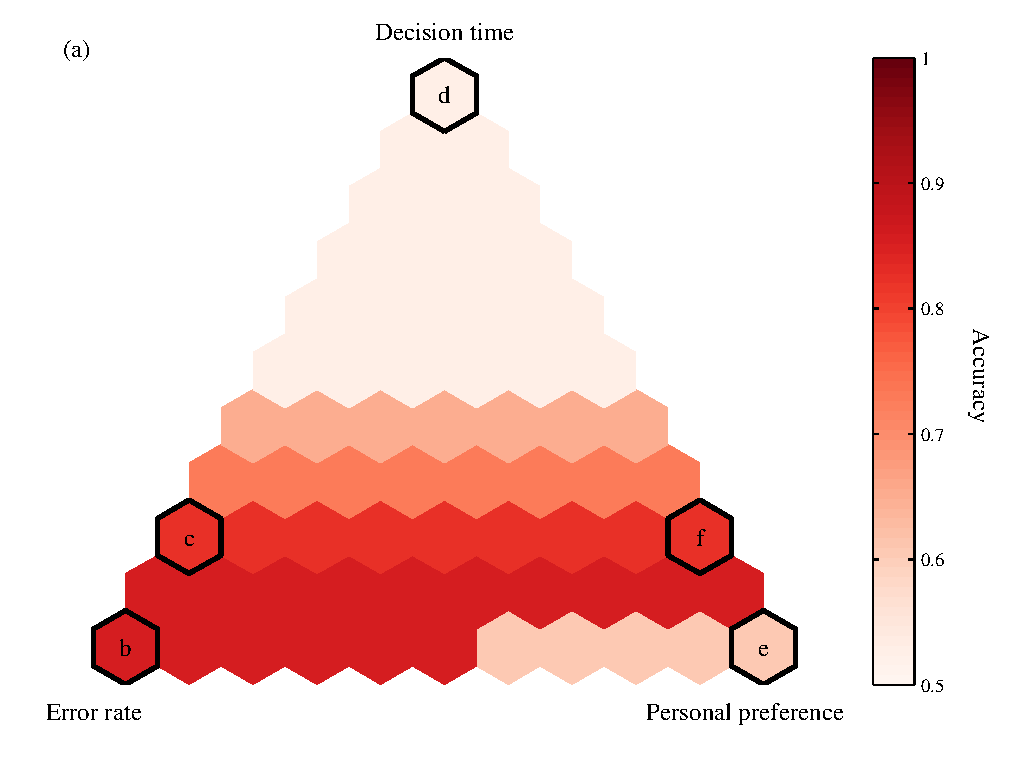
\includegraphics[width=\textwidth]{/Users/eleanorbrush/Dropbox/signaling_network/pairwise_accuracy.pdf}
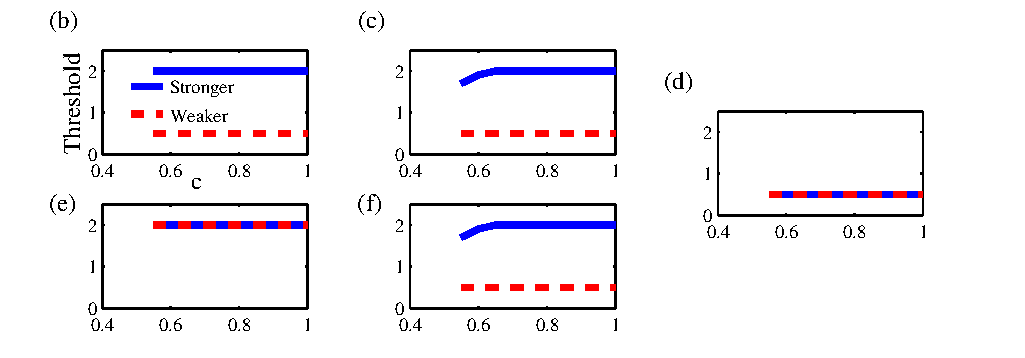
\includegraphics[width=\textwidth]{/Users/eleanorbrush/Dropbox/signaling_network/nasheq_thresholds.pdf}
\caption{\label{nasheq_thresholds}  The accuracy of a pair using Nash equilibrium thresholds decreases as the weight given to decision time increases.  (a) In the upper panel, the color indicates the accuracy of a decision made by a pair making a difficult decision ($c=.55$) using Nash equilibrium thresholds, as a function of the optimization weights, $w_1$, $w_2$, $w_3$.  In the lower left corner of the simplex, only error rate matters ($w_1=1$).  In the upper corner, only decision time matters ($w_2=1$).  In the lower right corner, only signaling probability matters ($w_3=1$). Accuracy decreases as $w_2$ increases but is not greatly affected by a tradeoff between $w_1$ and $w_3$. In (b)-(g) we show how the Nash equilibrium thresholds (top row) and decision time for a pair using those thresholds (bottom row) depends on the difficulty of the decision ($c$). The optimization weights for each panel are indicated in the simplex with the corresponding letter.  At intermediate waiting costs (f), intermediately difficult decision take the longest.}
\end{figure}

\begin{figure}
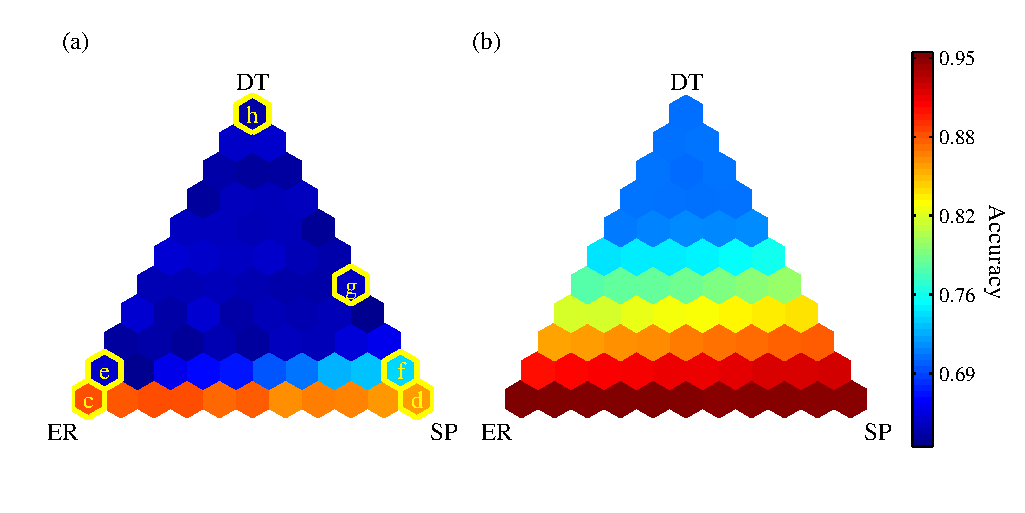
\includegraphics[width=\textwidth]{/Users/eleanorbrush/Dropbox/signaling_network/groupaccuracy_heatmap.pdf}
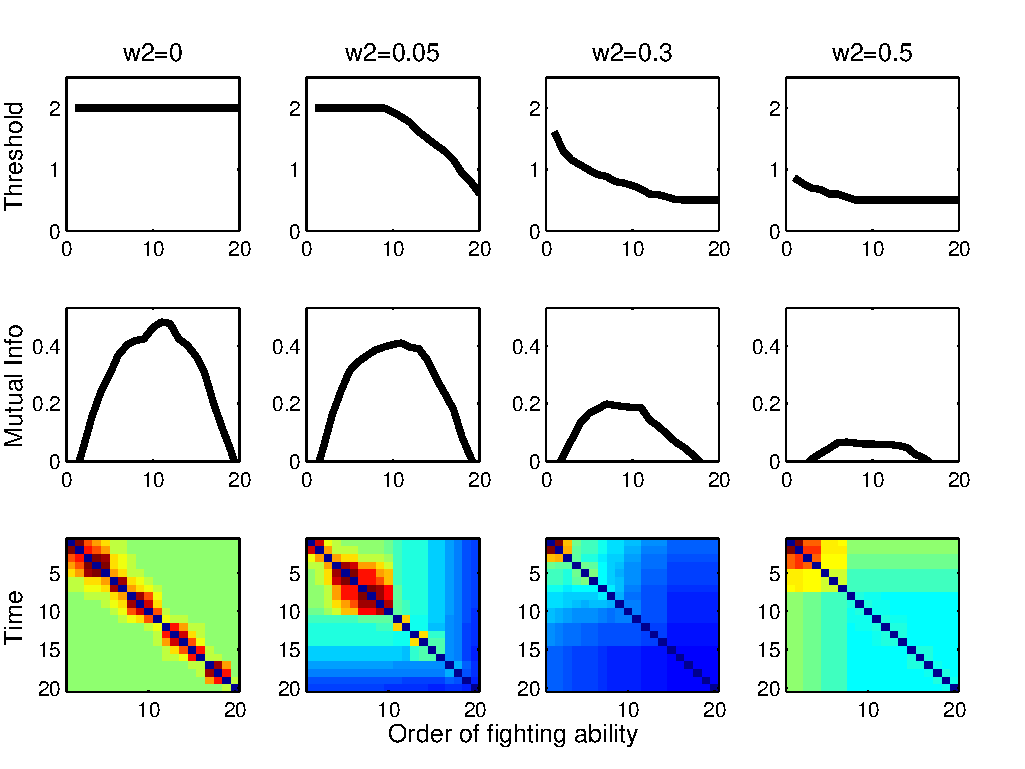
\includegraphics[width=\textwidth]{/Users/eleanorbrush/Dropbox/signaling_network/groupeq_thresholds.pdf}
\caption{\label{groupeq_thresholds}   The accuracy of a group using optimal thresholds decreases as the weight given to decision time increases.  In the upper panels, the color indicates the average accuracy of the decisions between individuals in the bottom quartile (a) and the average accuracy of the whole group (b) using optimal thresholds, as a function of the optimization weights, $w_1$, $w_2$, $w_3$.  In the lower left corner of the simplex, only error rate matters ($w_1=1$).  In the upper corner, only decision time matters ($w_2=1$).  In the lower right corner, only signaling probability matters ($w_3=1$). Both bottom-quartile and total accuracy decrease as $w_2$ increases, and the increase in bottom-quartile accuracy as $w_3$ increases drives a slight increase in total accuracy.  In (c)-(h) we show how the group-context optimal thresholds (top row) and decision time for each pair (bottom row) depends on the true order of ability where $1$ is the strongest animal and $20$ is the weakest. The optimization weights for each panel are indicated in the simplex with the corresponding letter.  For low waiting costs (c and d), it takes longest for pairs with similar ability to reach a decision.  For slightly higher waiting costs (f and g), it takes longer for pairs with similar and high ability to reach a decision.}
\end{figure}

\begin{figure}[ht]
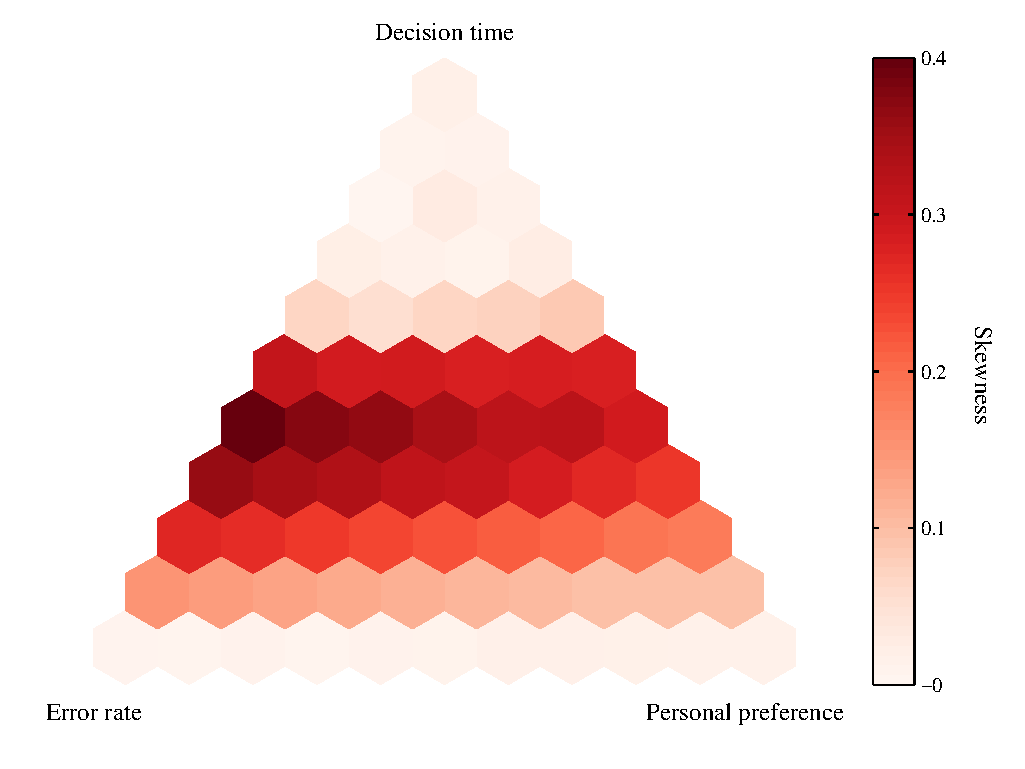
\includegraphics[width=\textwidth]{/Users/eleanorbrush/Dropbox/signaling_network/skewness_heatmap.pdf}
\caption{\label{skewness} The average skewness of the distribution of the number of signalers is maximized at intermediate waiting costs. In the lower left corner of the simplex, only error rate matters ($w_1=1$).  In the upper corner, only decision time matters ($w_2=1$).  In the lower right corner, only signaling probability matters ($w_3=1$).}
\end{figure}

\begin{figure}[ht]
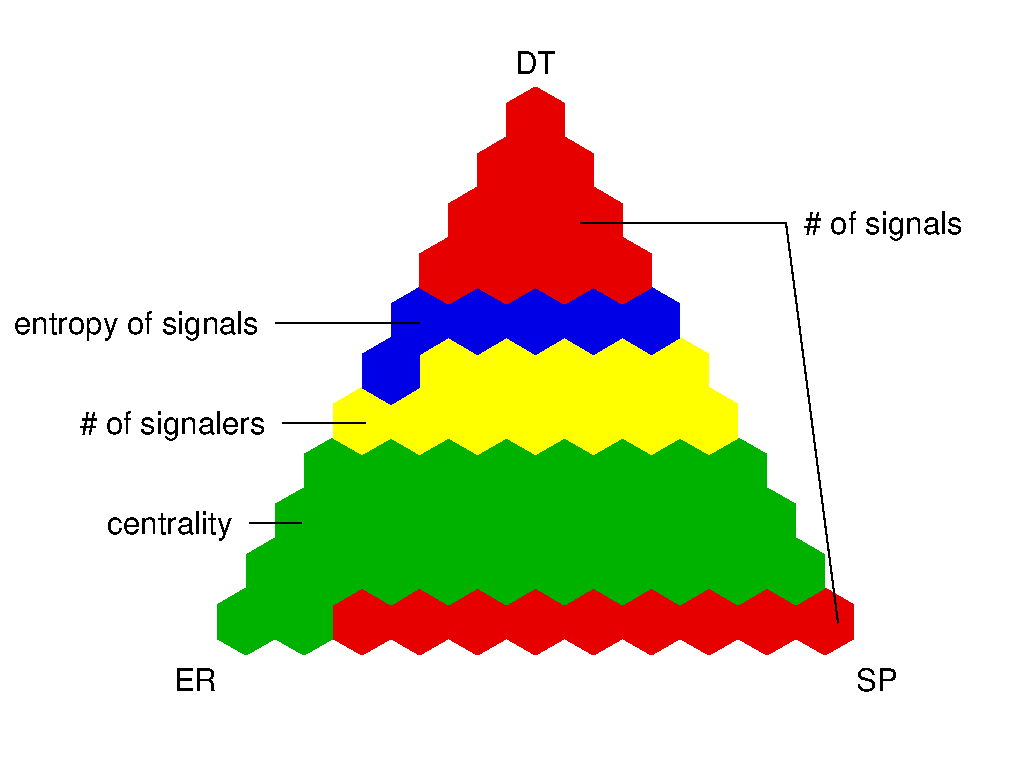
\includegraphics[width=\textwidth]{/Users/eleanorbrush/Dropbox/signaling_network/mostinformative_heatmap.pdf}
\caption{\label{bestmetric}  Which measure of consensus is most informative about fighting ability depends on how accurate decision are on average.  When decision are very accurate or very inaccurate, measures of the number of signals received are most informative.  When accuracy is slightly lower, eigenvector centrality of the signaling network is most informative.  When accuracy is slightly lower again, the number of signalers is most informative.  When accuracy is lower still, the entropy of signals received is most informative.  In the lower left corner of the simplex, only error rate matters ($w_1=1$).  In the upper corner, only decision time matters ($w_2=1$).  In the lower right corner, only signaling probability matters ($w_3=1$).}
\end{figure}

\begin{table}[ht]
\centering
\caption{\label{variables}{\bf  Variables and interpretations in neural and social systems.} }
\ra{1.3}
\begin{tabular}{@{}lllll@{}}
Variable & Interpretation & Neural &   Social \\
\cmidrule{1-4} 
& input & dots moving left or right & fights won or lost
\\$c$ & strength of input & coherence of dots & prob. of stronger animal winning
\\$X_1,X_2$ & decision variables &  firing rates of neural populations & opinions about relative dominance
\\ $w_1$ & error rate weight & reward from being ``right" & reward from being ``right"
\\ $w_2$ & decision time weight & penalty for taking a long time & costs of fighting
\\ $w_3$ & signaling prob. weight & ? & benefit from receiving signal
\\ & decision & subject indicates left or right & one animal emits subordination signal
\\ & correct decision & subject chooses correct direction & weaker animal signals
\end{tabular}
\end{table}

\begin{table}[ht]
\centering
\caption{\label{differences}{\bf  Comparison of models applied to neural and social systems.} Differences are highlighted in red.}
\ra{1.3}
\begin{tabular}{@{}lllll@{}}
& \multicolumn{2}{c}{Neural} &  Social \\
\cmidrule{2-3} \cmidrule{4-4} 
dimensionality & $1$  && $2$
\\decision & difference hits a threshold  && \fcolorbox{red}{white}{one var. hits a threshold}
\\ optimality criterion &  reward from being ``right" && reward from being ``right"
\\ & decision time && decision time
\\ & && \fcolorbox{red}{white}{reward from  receiving signal}
\\optimization depends on & input strength && input strength
\\ & noise && noise
\\ & leak rate && leak rate
\\ & && \fcolorbox{red}{white}{other animal's threshold}
\end{tabular}
\end{table}

\pagebreak
\section{Appendix}

\subsection{Derivation of PDEs for waiting time and accuracy \label{pdes_deriv}}

\pagebreak
\nocite{*}
\bibliographystyle{plain}
\bibliography{signaling_model}

\end{document}


